\documentclass[11pt]{article}

\usepackage[a4paper,margin=1in]{geometry}
\usepackage{amsmath}
\usepackage{amssymb}
\usepackage{booktabs}
\usepackage{pgfplots}
\usepackage{tikz}
\usepgfplotslibrary{groupplots}
\pgfplotsset{compat=1.17}

\pgfmathdeclarefunction{Uk}{2}{%
  \pgfmathparse{
    1
    + (#1-1)
      / (
        #2*#1
        * (
          1
          + sqrt(
            1
            + (
              4*(#1-1)
              * ((#1-1) + #2*(#1^2-2*#1+2))
            )
            / (#2*#1^2)
          )
        )
      )
  }%
}

\title{Computed Objective Maxima vs piecewise Lower-Bound}
\author{}
\date{}

\begin{document}



\section*{MINLP Formulation}

Fix \(m\in\mathbb{N}\), \(a\in(0,\frac12]\), \(b=1\), and let
\[
  I=\{(i,j): i,j=1,\ldots,m\}.
\]
The set \(I\) indexes the variables \(p_{ij}\). We define
one combined indexing set
\[
  K=I\cup\{L_1,\ldots,L_m\}
\]

The continuous decision variables are
\[
  p_{ij}\ge 0\quad ((i,j)\in I),\qquad
  l_i\ge 0\quad (i=1,\ldots,m),
\]
where \(p_{ij}\) denotes the size of the \(j\)-th listed job scheduled on
machine \(i\).  Thus \(p_{1j}\) and \(p_{2j}\) do not refer to the same
global job; the index \(j\) is local to each machine.

The binary assignment variables are
\[
  x_{kg}\in\{0,1\}\quad (k\in K,\;g=1,\ldots,m).
\]
Here \(x_{kg}=1\) means that item \(k\) is assigned to partition group
\(g\) (i.e machine g).  Define the value of each item by
\[
  v_{ij}=p_{ij}\quad ((i,j)\in I),
  \qquad
  v_{L_i}=l_i\quad (i=1,\ldots,m),
\]
and define the machine loads
\[
  P_g=\sum_{k\in K}x_{kg}v_k\qquad (g=1,\ldots,m).
\]
The model solved by SCIP is:
\[
\begin{aligned}
\max\quad
  & r \\[0.4em]
\text{s.t.}\quad
  & \sum_{j=1}^m p_{ij}=b
      && i=1,\ldots,m,\\[0.4em]
  & \sum_{g=1}^m x_{kg}=1
      && k\in K,\\[0.4em]
  & P_g=\sum_{k\in K}x_{kg}v_k
      && g=1,\ldots,m,\\[0.4em]
  & P_g\ge \epsilon
      && g=1,\ldots,m,\\[0.4em]
  & r\left(
      \sum_{g=1}^m P_g^2
      +(2a-1)\left(\sum_{i=1}^m\sum_{j=1}^m p_{ij}^2
      +\sum_{i=1}^m l_i^2\right)
    \right)\\
  &\hspace{5em}\le
    \sum_{i=1}^m(l_i+b)^2
    +(2a-1)\left(\sum_{i=1}^m\sum_{j=1}^m p_{ij}^2
    +\sum_{i=1}^m l_i^2\right),\\[0.4em]
  & \sum_{g=1}^m P_g^2
      +(2a-1)\left(\sum_{i=1}^m\sum_{j=1}^m p_{ij}^2
      +\sum_{i=1}^m l_i^2\right)
      \ge \epsilon,\\[0.4em]
  & 0\le p_{ij}\le b
      && i,j=1,\ldots,m,\\[0.4em]
  & 0\le l_i\le 30
      && i=1,\ldots,m,\\[0.4em]
  & 0\le r\le 1+\frac{1}{6a},\\[0.4em]
  & x_{kg}\in\{0,1\}
      && k\in K,\;g=1,\ldots,m.
\end{aligned}
\]

\begin{figure}[ht]
\centering

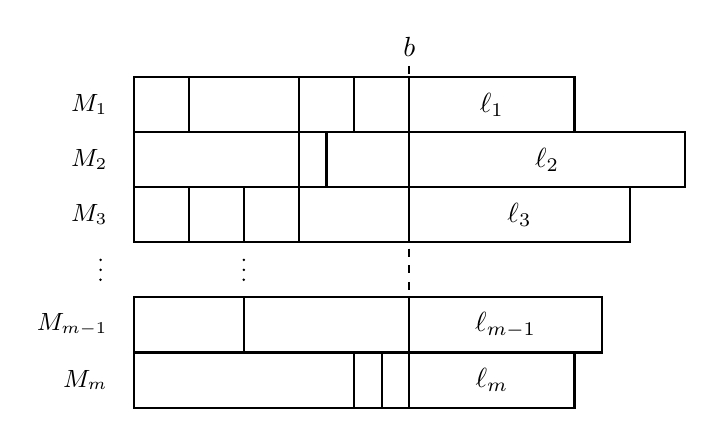
\begin{tikzpicture}[
    x=0.7cm,
    y=0.7cm,
    job/.style={
        draw,
        thick,
        fill=white,
        font=\small
    },
    machine/.style={font=\small}
]

% ------------------------------------------------
% Template idea:
% row      = displayed vertical row in the picture
% machine  = actual machine label shown on the left
%
% Use \machinerow{row}{machine label}
% Use \dotsrow{row}
% Use \jobblock{row}{start}{length}{job label}
% Use \jobblock[gray!25]{row}{start}{length}{job label} for shading
% ------------------------------------------------

\newcommand{\machinerow}[2]{
    \node[machine, anchor=east] at (-0.3,-#1+0.5) {$M_{#2}$};
}

\newcommand{\dotsrow}[1]{
    \foreach \dy in {-0.18,0,0.18} {
        \fill (-0.6,{-#1+0.5+\dy}) circle[radius=0.025];
        \fill (2,{-#1+0.5+\dy}) circle[radius=0.025];
    }
}

\newcommand{\jobblock}[5][white]{
    \draw[job, fill=#1] (#3,-#2) rectangle ++(#4,1);
    \node at ({#3 + #4/2},{-#2 + 0.5}) {$#5$};
}

% Displayed machine rows
\machinerow{1}{1}
\machinerow{2}{2}
\machinerow{3}{3}
\dotsrow{4}
\machinerow{5}{m-1}
\machinerow{6}{m}

% Example jobs
\jobblock{1}{0}{1}{}
\jobblock{1}{1}{2}{}
\jobblock{1}{3}{1}{}
\jobblock{1}{4}{1}{}
\jobblock{1}{5}{3}{\ell_1}

\jobblock{2}{0}{3}{}
\jobblock{2}{3}{0.5}{}
\jobblock{2}{3.5}{1.5}{}
\jobblock{2}{5}{5}{\ell_2}

\jobblock{3}{0}{1}{}
\jobblock{3}{1}{1}{}
\jobblock{3}{2}{1}{}
\jobblock{3}{3}{2}{}
\jobblock{3}{5}{4}{\ell_3}

\jobblock{5}{0}{2}{}
\jobblock{5}{2}{3}{}
\jobblock{5}{5}{3.5}{\ell_{m-1}}

\jobblock{6}{0}{4}{}
\jobblock{6}{4}{0.5}{}
\jobblock{6}{4.5}{0.5}{}
\jobblock{6}{5}{3}{\ell_m}

% Timestamp marker where all \ell jobs begin
\draw[dashed, thick] (5,0.2) -- (5,-6.0);
\node[above] at (5,0.2) {$b$};

\end{tikzpicture}

\caption{MINLP is restricted to $S_W$ schedules of this form. The determination of $S^*$ is free for the algorithm to choose.}
\label{fig:computational-schedule-structure}

\end{figure}
\begin{center}
\begin{tikzpicture}
\begin{axis}[
  width=0.94\textwidth,
  height=0.67\textheight,
  xmode=log,
  log basis x=10,
  x dir=reverse,
  xmin=0.001111111111,
  xmax=0.5,
  ymin=1,
  ymax=17,
  xlabel={Parameter \(a\)},
  ylabel={Objective value},
  xtick={
    0.5,
    0.1,
    0.02,
    0.005,
    0.0025,
    0.001111111111
  },
  xticklabels={
    \(\frac12\),
    \(\frac1{10}\),
    \(\frac1{50}\),
    \(\frac1{200}\),
    \(\frac1{400}\),
    \(\frac1{900}\)
  },
  grid=both,
  major grid style={gray!35},
  minor grid style={gray!15},
  legend style={
    at={(0.5,-0.17)},
    anchor=north,
    legend columns=3,
    draw=none
  },
  tick label style={font=\small},
  label style={font=\large},
]

% Breakpoints a_k=1/D_k, where D_k=k^4-2k^3-2k^2+k+3.
\addplot[gray,dashed,forget plot] coordinates {(0.066666666667,1) (0.066666666667,17)};
\node[anchor=south,fill=white,inner sep=1pt] at (axis cs:0.066666666667,16.3)
  {\(a_3\)};

\addplot[gray,dashed,forget plot] coordinates {(0.009708737864,1) (0.009708737864,17)};
\node[anchor=south,fill=white,inner sep=1pt] at (axis cs:0.009708737864,16.3)
  {\(a_4\)};

\addplot[gray,dashed,forget plot] coordinates {(0.003003003003,1) (0.003003003003,17)};
\node[anchor=south,fill=white,inner sep=1pt] at (axis cs:0.003003003003,16.3)
  {\(a_5\)};

\addplot[gray,dashed,forget plot] coordinates {(0.001248439451,1) (0.001248439451,17)};
\node[anchor=south,fill=white,inner sep=1pt] at (axis cs:0.001248439451,16.3)
  {\(a_6\)};

% Piecewise branches of U_k(a).
\addplot[blue!75!black,very thick,domain=0.066666666667:0.5,samples=100]
  {Uk(3,x)};
\addlegendentry{\(U_3(a)\)}

\addplot[teal!80!black,very thick,domain=0.009708737864:0.066666666667,samples=100]
  {Uk(4,x)};
\addlegendentry{\(U_4(a)\)}

\addplot[green!55!black,very thick,domain=0.003003003003:0.009708737864,samples=100]
  {Uk(5,x)};
\addlegendentry{\(U_5(a)\)}

\addplot[orange!90!black,very thick,domain=0.001248439451:0.003003003003,samples=100]
  {Uk(6,x)};
\addlegendentry{\(U_6(a)\)}

\addplot[purple!80!black,very thick,domain=0.001111111111:0.001248439451,samples=100]
  {Uk(7,x)};
\addlegendentry{\(U_7(a)\)}

% At each a, this is max over the computed m=3,...,7 objectives.
\addplot[
  only marks,
  mark=*,
  mark size=3.2pt,
  red!85!black,
  fill=red!65,
] coordinates {
  (0.5,          1.333333346656501)
  (0.1,          2.145683320593890)
  (0.02,         4.118401735799101)
  (0.005,        7.694623551818327)
  (0.0025,      10.642889269095093)
  (0.001111111111,15.644793715614036)
};
\addlegendentry{\(\max_{m=3,\ldots,7}\) computed objective}

% Visible vertical gaps between the curve and computed points.
\addplot[red!70!black,thick,forget plot] coordinates {
  (0.02,4.118401735799101)
  (0.02,4.125000000000000)
};
\addplot[red!70!black,thick,forget plot] coordinates {
  (0.005,7.694623551818327)
  (0.005,7.697804474378321)
};
\addplot[red!70!black,thick,forget plot] coordinates {
  (0.0025,10.642889269095093)
  (0.0025,10.643889586940004)
};
\addplot[red!70!black,thick,forget plot] coordinates {
  (0.001111111111,15.644793715614036)
  (0.001111111111,15.661998372367162)
};



\end{axis}
\end{tikzpicture}
\end{center}

\begin{center}
\small
\emph{Parameter values}
\(b=1\), \(0\le l_i\le 30\), SCIP node limit \(=20000\), and
\(\epsilon=10^{-5}\).
\end{center}

\newpage
\section*{Differences}

\noindent
Let
\[
  \Delta(a)=U(a)-\max_{m=3,\ldots,7}F_m(a).
\]
At \(a=\frac12\) and \(a=\frac1{10}\), the computed values exceed
\(U(a)\) only by \(1.3\cdot10^{-8}\) and \(9.1\cdot10^{-8}\),
respectively. So they are displayed below as \(\Delta(a)\approx0\).

\begin{center}
\begin{tikzpicture}
\begin{axis}[
  ybar,
  width=0.9\textwidth,
  height=0.48\textheight,
  ymin=0,
  ymax=0.019,
  ylabel={\(\Delta(a)\)},
  symbolic x coords={
    {$\frac12$},
    {$\frac1{10}$},
    {$\frac1{50}$},
    {$\frac1{200}$},
    {$\frac1{400}$},
    {$\frac1{900}$}
  },
  xtick=data,
  bar width=18pt,
  nodes near coords,
  nodes near coords style={
    font=\small,
    /pgf/number format/fixed,
    /pgf/number format/precision=6
  },
  grid=major,
  major grid style={gray!25},
  enlarge x limits=0.08,
]
\addplot[fill=blue!45,draw=blue!75!black] coordinates {
  ({$\frac12$},0)
  ({$\frac1{10}$},0)
  ({$\frac1{50}$},0.006598264201)
  ({$\frac1{200}$},0.003180922560)
  ({$\frac1{400}$},0.001000317845)
  ({$\frac1{900}$},0.017204656753)
};
\end{axis}
\end{tikzpicture}
\end{center}

\begin{center}
\begin{tikzpicture}
\begin{groupplot}[
  group style={group size=2 by 2,horizontal sep=1.2cm,vertical sep=2.2cm},
  width=0.42\textwidth,
  height=0.22\textheight,
  grid=major,
  major grid style={gray!20},
  xlabel={\(a\)},
  ylabel={Objective},
  tick label style={font=\scriptsize},
  label style={font=\small},
]
\nextgroupplot[
  title={Near \(a=\frac1{50}\)},
  xmin=0.0195,xmax=0.0205,
  ymin=4.116,ymax=4.127,
]
\addplot[green!55!black,very thick,domain=0.0195:0.0205,samples=50] {Uk(4,x)};
\addplot[only marks,mark=*,red,mark size=3pt] coordinates {(0.02,4.118401735799101)};

\nextgroupplot[
  title={Near \(a=\frac1{200}\)},
  xmin=0.00485,xmax=0.00515,
  ymin=7.692,ymax=7.700,
]
\addplot[green!55!black,very thick,domain=0.00485:0.00515,samples=50] {Uk(5,x)};
\addplot[only marks,mark=*,red,mark size=3pt] coordinates {(0.005,7.694623551818327)};

\nextgroupplot[
  title={Near \(a=\frac1{400}\)},
  xmin=0.00243,xmax=0.00257,
  ymin=10.6415,ymax=10.6452,
]
\addplot[orange!90!black,very thick,domain=0.00243:0.00257,samples=50] {Uk(6,x)};
\addplot[only marks,mark=*,red,mark size=3pt] coordinates {(0.0025,10.642889269095093)};

\nextgroupplot[
  title={Near \(a=\frac1{900}\)},
  xmin=0.00109,xmax=0.001135,
  ymin=15.64,ymax=15.67,
]
\addplot[purple!80!black,very thick,domain=0.00109:0.001135,samples=50] {Uk(7,x)};
\addplot[only marks,mark=*,red,mark size=3pt] coordinates {(0.001111111111,15.644793715614036)};
\end{groupplot}
\end{tikzpicture}
\end{center}

\end{document}
